% Created 2021-10-15 Fri 07:39
% Intended LaTeX compiler: pdflatex
\documentclass[presentation,aspectratio=169]{beamer}
\usepackage[utf8]{inputenc}
\usepackage[T1]{fontenc}
\usepackage{graphicx}
\usepackage{grffile}
\usepackage{longtable}
\usepackage{wrapfig}
\usepackage{rotating}
\usepackage[normalem]{ulem}
\usepackage{amsmath}
\usepackage{textcomp}
\usepackage{amssymb}
\usepackage{capt-of}
\usepackage{hyperref}
\usepackage{pifont}
\newcommand{\cmark}{\textcolor{green!80!black}{\ding{51}}}
\usepackage{amssymb}
\usepackage{pgfplotstable}
\DeclareMathOperator{\shift}{q}
\DeclareMathOperator{\diff}{p}
\usepackage{khpreamble, euscript, mathtools}
\DeclareMathOperator{\atantwo}{atan2}
\newcommand*{\ctrb}{\EuScript{C}}
\newcommand*{\obsv}{\EuScript{O}}
\usetheme{default}
\author{Kjartan Halvorsen}
\date{\today}
\title{State feedback}
\hypersetup{
 pdfauthor={Kjartan Halvorsen},
 pdftitle={State feedback},
 pdfkeywords={},
 pdfsubject={},
 pdfcreator={Emacs 26.3 (Org mode 9.4.6)}, 
 pdflang={English}}
\begin{document}

\maketitle



\section{Apollo moon lander}
\label{sec:orgf2ea2b4}

\begin{frame}[label={sec:org348834a}]{The Apollo lunar module}
\begin{center}
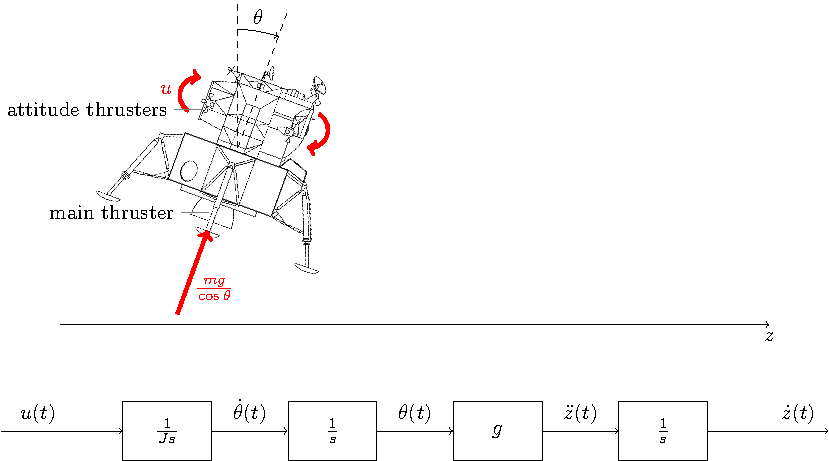
\includegraphics[width=0.7\linewidth]{../../figures/fig-apollo}
\end{center}

\pause

\alert{Activity} Which is the transfer function of the system?
   \[1: \; G(s) = \frac{\frac{g}{J} }{s^2}\qquad 2: \; G(s) = \frac{\frac{g}{J} }{s(s^2 + 1)} \qquad 3: \; G(s) = \frac{\frac{g}{J} }{s^3}\]
\end{frame}



\begin{frame}[label={sec:orgfaa9732}]{State variables}
\begin{columns}
\begin{column}{0.65\columnwidth}
\begin{center}
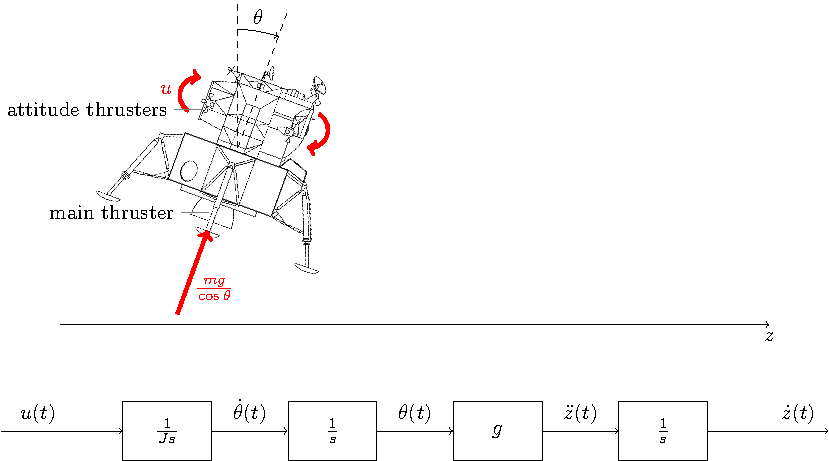
\includegraphics[width=\linewidth]{../../figures/fig-apollo}
\end{center}

State variables: \(x = \begin{bmatrix} x_1 & x_2 & x_3 \end{bmatrix}^T = \begin{bmatrix} \dot{\theta} & \theta & \dot{z} \end{bmatrix}^T\).
\end{column}

\begin{column}{0.45\columnwidth}
With dynamics
  \[ \begin{cases} \dot{x}_1 =  \ddot{\theta} = \frac{1}{J} u\\ \dot{x}_2 = \dot{\theta} = x_1\\ \dot{x}_3 = \ddot{z} = g\theta = gx_2 \end{cases} \]
\end{column}
\end{columns}
\end{frame}

\begin{frame}[label={sec:orgc9f7ee6}]{State-space model}
State variables: \(x = \begin{bmatrix} x_1 & x_2 & x_3 \end{bmatrix}^T = \begin{bmatrix} \dot{\theta} & \theta & \dot{z} \end{bmatrix}^T\). With dynamics
\[ \begin{cases} \dot{x}_1 =  \ddot{\theta} = \frac{1}{J} u\\ \dot{x}_2 = \dot{\theta} = x_1\\ \dot{x}_3 = \ddot{z} = g\theta = gx_2 \end{cases} \]

\alert{Activity} Fill the matrix \(A\) and vector \(B\).

\[ \dot{x} = \begin{bmatrix} \dot{x}_1\\\dot{x}_2\\\dot{x}_3\end{bmatrix} = \underbrace{\begin{bmatrix} \textcolor{white}{0} & \textcolor{white}{0} &\textcolor{white}{0} \\\textcolor{white}{1} & \textcolor{white}{0}& \textcolor{white}{0}\\ \textcolor{white}{0}& \textcolor{white}{g} &\textcolor{white}{0} \end{bmatrix}}_{A} \begin{bmatrix} x_1\\x_2\\x_3\end{bmatrix} + \underbrace{\begin{bmatrix} \textcolor{white}{\frac{1}{J}} \\ \textcolor{white}{0} \\\textcolor{white}{0}  \end{bmatrix}}_{B} u \]
\end{frame}

\begin{frame}[label={sec:org0597e2b}]{State-space model}
\end{frame}
\begin{frame}[label={sec:org2af19a2}]{State-space model}
State variables: \(x = \begin{bmatrix} x_1 & x_2 & x_3 \end{bmatrix}^T = \begin{bmatrix} \dot{\theta} & \theta & \dot{z} \end{bmatrix}^T\). With dynamics
\[ \begin{cases} \dot{x}_1 =  \ddot{\theta} = \frac{1}{J} u\\ \dot{x}_2 = \dot{\theta} = x_1\\ \dot{x}_3 = \ddot{z} = g\theta = gx_2 \end{cases} \]

\[ \dot{x} = \begin{bmatrix} \dot{x}_1\\\dot{x}_2\\\dot{x}_3\end{bmatrix} = \underbrace{\begin{bmatrix} \textcolor{red!60!black}{0} & \textcolor{red!60!black}{0} &\textcolor{red!60!black}{0} \\\textcolor{red!60!black}{1} & \textcolor{red!60!black}{0}& \textcolor{red!60!black}{0}\\ \textcolor{red!60!black}{0}& \textcolor{red!60!black}{g} &\textcolor{red!60!black}{0} \end{bmatrix}}_{A} \begin{bmatrix} x_1\\x_2\\x_3\end{bmatrix} + \underbrace{\begin{bmatrix} \textcolor{red!60!black}{\frac{1}{J}} \\ \textcolor{red!60!black}{0} \\\textcolor{red!60!black}{0}  \end{bmatrix}}_{B} u \]

\pause

\alert{Activity} What are the poles of the system?
\end{frame}

\begin{frame}[label={sec:org76223fa}]{Sensors}
\begin{center}
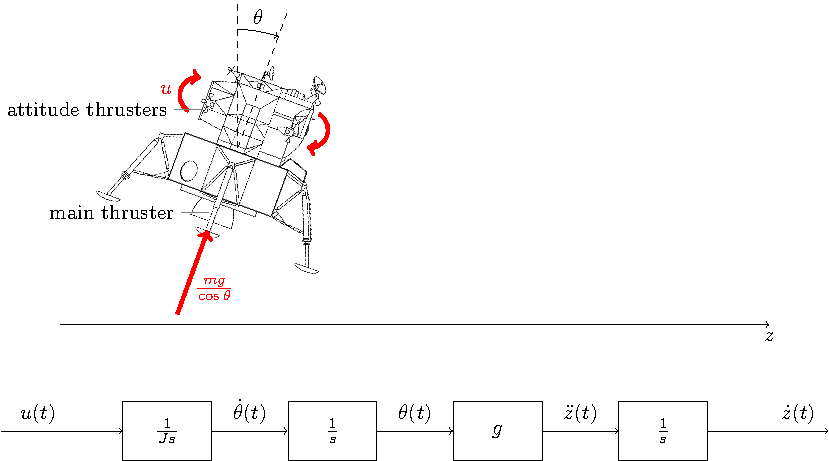
\includegraphics[width=0.8\linewidth]{../../figures/fig-apollo}
\end{center}
\alert{Activity} What sensors are needed for state feedback?
\end{frame}

\begin{frame}[label={sec:orgb7c22f6}]{Controllability}
\[ \dot{x} = \begin{bmatrix} \dot{x}_1\\\dot{x}_2\\\dot{x}_3\end{bmatrix} = \underbrace{\begin{bmatrix} \textcolor{black!60!black}{0} & \textcolor{black!60!black}{0} &\textcolor{black!60!black}{0} \\\textcolor{black!60!black}{1} & \textcolor{black!60!black}{0}& \textcolor{black!60!black}{0}\\ \textcolor{black!60!black}{0}& \textcolor{black!60!black}{g} &\textcolor{black!60!black}{0} \end{bmatrix}}_{A} \begin{bmatrix} x_1\\x_2\\x_3\end{bmatrix} + \underbrace{\begin{bmatrix} \textcolor{black!60!black}{\frac{1}{J}} \\ \textcolor{black!60!black}{0} \\\textcolor{black!60!black}{0}  \end{bmatrix}}_{B} u \]

Forming the controllability matrix. Note that
\[ A^2 = \begin{bmatrix} 0 &  0 & 0\\ 0 & 0 & 0\\ g & 0 & 0 \end{bmatrix} \]
\[ \mathcal{C} = \begin{bmatrix} B & AB & A^2B\end{bmatrix}
   = \begin{bmatrix} \frac{1}{J} & 0 & \textcolor{white}{0}\\0 & \frac{1}{J} & \textcolor{white}{0} \\0 & 0 & \textcolor{white}{\frac{1}{J}g} \end{bmatrix} \]

\pause
\alert{Activity} Is the system controllable?
\end{frame}


\begin{frame}[label={sec:org827db36}]{Linear state feedback}
\begin{columns}
\begin{column}{0.6\columnwidth}
\[ \dot{x} = \begin{bmatrix} \dot{x}_1\\\dot{x}_2\\\dot{x}_3\end{bmatrix} = \underbrace{\begin{bmatrix} \textcolor{black!60!black}{0} & \textcolor{black!60!black}{0} &\textcolor{black!60!black}{0} \\\textcolor{black!60!black}{1} & \textcolor{black!60!black}{0}& \textcolor{black!60!black}{0}\\ \textcolor{black!60!black}{0}& \textcolor{black!60!black}{g} &\textcolor{black!60!black}{0} \end{bmatrix}}_{A} \begin{bmatrix} x_1\\x_2\\x_3\end{bmatrix} + \underbrace{\begin{bmatrix} \textcolor{black!60!black}{\frac{1}{J}} \\ \textcolor{black!60!black}{0} \\\textcolor{black!60!black}{0}  \end{bmatrix}}_{B} u \]

Introduce linear state feedback

\[ u = -\textcolor{morange}{L}x + \textcolor{mbluegreen}{l_0} r,\]
where \(r\) is a reference signal.
\end{column}

\begin{column}{0.4\columnwidth}
Closed-loop system

\[\dot{x} = (A-B\textcolor{morange}{L})x + \textcolor{mbluegreen}{l_0}Br\]

Since the system is \alert{controllable}, we can find a gain vector \(\textcolor{morange}{L}\) that places the eigenvalues of \(A-B\textcolor{morange}{L}\) (the poles of the closed-loop system) at desired locations.
\end{column}
\end{columns}
\end{frame}

\begin{frame}[label={sec:org17d03c2}]{Linear state feedback}
\small

The poles of 
\(\dot{x} = (A-B\textcolor{morange}{L})x + \textcolor{mbluegreen}{l_0}Br\)
are given by the solutions to the characteristic equation

\begin{align*}
\det \Big(sI - (A-B\textcolor{morange}{L})\Big) &= 0\\
\det \left(\begin{bmatrix} s & 0 & 0\\ 0 & s & 0\\ 0 & 0 & s
\end{bmatrix}
- \begin{bmatrix} 0 & 0 & 0\\1 & 0 & 0\\0 & g & 0\end{bmatrix}
+ \begin{bmatrix} \frac{1}{J}\textcolor{morange}{l_1} & \frac{1}{J}\textcolor{morange}{l_2} & \frac{1}{J}\textcolor{morange}{l_3}\\0 & 0 & 0\\0 & 0 & 0\end{bmatrix}\right) &= 0\\
\det \begin{bmatrix} s+\frac{1}{J}\textcolor{morange}{l_1} & \frac{1}{J}\textcolor{morange}{l_2} & \frac{1}{J}\textcolor{morange}{l_3}\\-1 & s & 0\\0 & -g & s \end{bmatrix} &= 0\\
(s+\frac{1}{J}\textcolor{morange}{l_1})s^2  + \frac{1}{J}\textcolor{morange}{l_2}s +\frac{1}{J}g\textcolor{morange}{l_3} &= 0\\
s^3 + \frac{1}{J}\textcolor{morange}{l_1}s^2 + \frac{1}{J}\textcolor{morange}{l_2}s +\frac{1}{J}g\textcolor{morange}{l_3} &= 0
\end{align*}
\end{frame}

\begin{frame}[label={sec:orga0df4f2}]{Where to place the closed-loop poles}
\begin{columns}
\begin{column}{0.35\columnwidth}
\begin{center}
  \begin{tikzpicture}[scale=0.7]
  \pgfmathsetmacro{\wc}{2}
  \pgfmathsetmacro{\rp}{\wc*cos(45)}
    \draw[->] (-4,0) to (2,0) node[below] {Re};
    \draw[->] (0,-3) to (0,3) node[left] {Im};

    \draw[dashed, black!80] (0,\wc) arc[radius=\wc{}cm, start angle=90, end angle=270]; 

    \node[anchor=center, red!80!black] at (-\rp, \rp) {\Large $\times$ };
    \node[anchor=center, red!80!black] at (-\rp, -\rp) {\Large $\times$ };
    \node[anchor=center, red!80!black] at (-\wc, 0) {\Large $\times$ };

    \draw[thin, <->] (0,0) -- node[above] {$\frac{1}{\tau_c}$} (-\rp, \rp);
    \end{tikzpicture}
\end{center}
\end{column}


\begin{column}{0.65\columnwidth}
Desired closed-loop characteristic polynomial

\begin{align*}
  (s-p_1)(s-p_2)(s-p_3) &= (s+\frac{1}{\tau_c})(s^2 + \frac{\sqrt{2}}{\tau_c}s + \frac{1}{\tau_c^2})\\
   &= s^3 + \frac{1 + \sqrt{2}}{\tau_c}s^2 + \frac{1+\sqrt{2}}{\tau_c^2}s + \frac{1}{\tau_c^3}
\end{align*}
\end{column}
\end{columns}
\end{frame}

\begin{frame}[label={sec:org6f6ed56}]{Determining the state feedback gain}
By linear state feedback we have characteristic polynomial
\[\det \Big(sI - (A-B\textcolor{morange}{L})\Big) =  s^3 + \frac{1}{J}\textcolor{morange}{l_1}s^2 + \frac{1}{J}\textcolor{morange}{l_2}s + \frac{1}{J}g\textcolor{morange}{l_3}.\]

And we want to achieve the characteristic polynomial
\[ s^3 + \frac{1 + \sqrt{2}}{\tau_c}s^2 + \frac{1+\sqrt{2}}{\tau_c^2}s + \frac{1}{\tau_c^3}. \]

\alert{Activity} What do we do next?
\end{frame}

\begin{frame}[label={sec:org2393acf}]{Determining the state feedback gain}
Set the characteristic polynomial obtained from \(\det\) \Big(sI - (A-B\textcolor{morange}{L})\Big) equal to the desired characteristic polynomial

\[ s^3 + \frac{1}{J}\textcolor{morange}{l_1}s^2 + \frac{1}{J}\textcolor{morange}{l_2}s + \frac{1}{J}g\textcolor{morange}{l_3} =  s^3 + \frac{1 + \sqrt{2}}{\tau_c}s^2 + \frac{1+\sqrt{2}}{\tau_c^2}s + \frac{1}{\tau_c^3} \]

Solve for the gains by setting corresponding coefficients equal.

\begin{equation*}
\begin{rcases}
s^2: \quad & \frac{1}{J}\textcolor{morange}{l_1} = \frac{1 + \sqrt{2}}{\tau_c}\\
s^1: \quad & \frac{1}{J}\textcolor{morange}{l_2} = \frac{1 + \sqrt{2}}{\tau_c^2}\\
s^0: \quad & \frac{1}{J}g\textcolor{morange}{l_3} = \frac{1}{\tau_c^3}
\end{rcases} \Rightarrow
\begin{rcases}
 \quad \textcolor{morange}{l_1} &= \frac{J(1 + \sqrt{2})}{\tau_c}\\
 \quad \textcolor{morange}{l_2} &= \frac{J(1 + \sqrt{2})}{\tau_c^2}\\
 \quad \textcolor{morange}{l_3} &= \frac{J}{g\tau_c^3}
\end{rcases}
\end{equation*}
\end{frame}


\begin{frame}[label={sec:org8879e69}]{The gain \(l_0\)}
\begin{center}
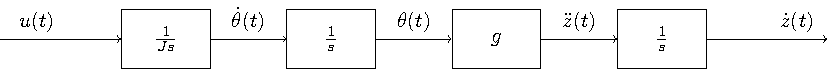
\includegraphics[width=0.6\linewidth]{../../figures/block-apollo}
\end{center}

\[ G(s) = \frac{\frac{g}{J}}{s^3}\]
It can be shown that state feedback does not change the numerator of the transfer function, only the denominator, so

\[G_c(s) = \textcolor{mbluegreen}{l_0}\frac{\frac{g}{J}}{s^3 + \frac{1 + \sqrt{2}}{\tau_c}s^2 + \frac{1+\sqrt{2}}{\tau_c^2}s + \frac{1}{\tau_c^3}}\]

We want unit static gain,  \(G_c(0) = 1\)

\pause

\alert{Activity} Determine the gain \(\textcolor{mbluegreen}{l_0}\)
\end{frame}
\end{document}